\documentclass[12pt]{extarticle}
\usepackage{fancyhdr,amsfonts,graphicx,wrapfig,sidecap,float,adjustbox,subcaption,indentfirst,amsmath,hyperref}
\usepackage{listings}
\usepackage{color}
\usepackage{gensymb}

\usepackage[right=2.5cm,left=2.5cm,top=2.5cm,bottom=2.5cm]{geometry}

\pagestyle{fancy}
\lhead{Memorial University of Newfoundland}
\rhead{Department of Mathematics and Statistics}
\renewcommand{\headrulewidth}{0.4pt}

\lfoot{Mathematics 2130}
\cfoot{}
\rfoot{Fall 2015, Project 4}
\renewcommand{\footrulewidth}{0.4pt}
\flushbottom
\begin{document}
\begin{titlepage}
\vspace*{2in}
\begin{center}
{\LARGE Road Traffic Simulation}
\end{center}

\vspace{2cm}

\abstract{This paper provides analysis of traffic flows. Its flow and density are a the main focus. The affects of gradual increased and decreased probabilities of deceleration and random stopping is also observed. These topics are analyzed and discussed in detail. }

\vspace{3in}
\begin{flushright}
\begin{tabular}{l}
Project 4 \\
Mathematics 2130\\
Submitted by: John Hollett\\
Submitted to: Ivan Booth\\
\today
\end{tabular}
\end{flushright}


\end{titlepage}


\lhead{Road Traffic Simulation}
\rhead{Math 2130}
\lfoot{John Hollett}
\rfoot{\thepage}

%\underheadoverfoot




\section{Introduction}

In this paper, a mathematical model is used to examine the characteristics of traffic flow. The model is a simplified example of real world traffic. For the purposes of this paper, traffic is defined as vehicles interacting on a road. The mathematical model utilizes mechanical processes that remove complexity from real world traffic and simplify it to provide results.

This mathematical model is set out with the programming language C$^\#$. The structure and inner mechanics will be discussed later in this paper. In the next section, the mechanics used to create the mathematical model used to carry out the analysis is explained. The goal of the analysis is to provide a better understanding of traffic flow and deadlocks that occurs. Using graphics and the simulation, the analysis performed will provide convincing evidence that the actions of drivers can influence reverberating traffic conditions.

\section{Mechanics}

The traffic model used consists of cars and roads. The road can be thought of as similar to a roundabout. This means that the road is an infinite loop. All vehicles are located on a road where they interact. Unlike in the real world, the cars in this simulation cannot cause accidents. 

The position of the cars is described by:
\begin{align}
\label{e1}
x_{i-1}(t) < x_{i}(t) < x_{i+1}(t)
\end{align}
Where $x$ is the car, $i$ is the index and $t$ is the time in the sequence. This rule is important to maintain consistent behavior amongst all cars. Without this rule, cars would collide and results would be inconsistent. 

The extent to which cars move and their density is described by:
\begin{align}
\label{e2}
& v_i(t) \in \{0,1,2, ..., V_{max}\} \\
\label{e3}
& D(C,R) = \frac{C}{R}
\end{align}
Where $v$ is the velocity of the car at index $i$. The speed of a car is an integer value and the maximum speed is described by $V_{max}$. Density is defined as cars divided by the length of road. Similar to real world traffic, in this model vehicles explicitly obey the speed limit. Cars will accelerate when possible and decelerate to avoid accidents. Each one has a probability for random deceleration. 

The rules of acceleration and deceleration are as follows:

\begin{align}
\notag A)& \ \ v_i(t) < V_{max} : v_i(t+1) = v_i(t) + 1\\ 
\notag B)& \ \  x_i(t) + v_i(t + 1) \geq x_{x+1}(t) : v_i(t + 1) =x_{i+1}(t) - x_i(t) - 1\\
\label{e4}
C)& \ \ Pr(P < P_{o}) :v_i(t+1) = v_i(t+1) - 1 
\end{align}

The rules above, in the order listed, are applied to each car in the simulation. When the new values are found, the position of each car is updated. This is achieved using the formula:
\begin{align}
\label{e5}
 x_i(t + 1) = x_i(t) + v_i(t+1)
\end{align}
Where $x$,$v$ and $t$ are position, velocity and time respectively; $i$ is the car in the list. The rules listed were assembled within a program and used to simulate road conditions. The next section will discuss the results of a number of tests that were carried out..

\section{Analysis}

The first test show the affect of density on cars while the second examines the probability of random deceleration. This is carried out by adjusting the probability of deceleration and density using equation (\ref{e3}) and (\ref{e4}). The third test examines the probability of deceleration increases and decreases on a section of road. Graphs are based on a simulation ran for 10,000 steps before data is gathered.

\subsection{Density Analysis}
\begin{figure}[h!]
	\centering
	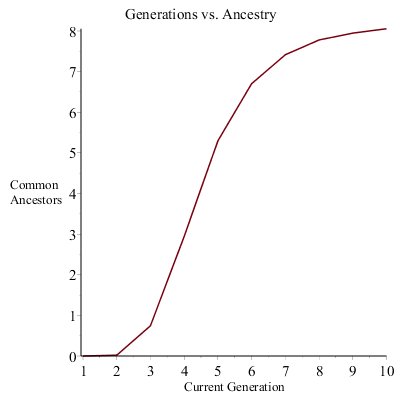
\includegraphics[scale=0.70]{Graph1.png}
	\caption{Cars = 200, Roads = 1,000, Prob = 0.05}
	\label{fig:img1}
\end{figure}


In the first test, the affect of density is examined. To do this effectively, the length of road and number of cars are chosen to maximize the data. An arbitrary road length of 1,000 was derived. Using equation (\ref{e3}), the density is set at 20\%. The number of cars derived from the equation is 200. To give the data character, the probability of deceleration is set at 5\%. The reasoning behind this is explained in the section containing technical details.

Figure (\ref{fig:img1}), shows the results. The colors \{black, red, orange, yellow, green, blue\} reflect the speed of the cars from 0 to 5. This color scheme used for all tests illustrated in this paper. The data show streaks of red and black diagonally aligned. This effect results from random deceleration of the cars. The x and y axis describes road segments and time respectively and the colors depict the velocities of individual cars.

The results of the first test performed are seen in figure (\ref{fig:img1}) which shows streaks of red which indicate consistent traffic jams over time. As time increases instances occur where traffic forms and dissipates seen as black and red in the figure. The difference between these two factors is consistent and inconsistent traffic jams. These are result of a probability that cars decelerate once or twice and this affects the following cars. Cars that decelerate to avoid collision also have a probability of deceleration decreasing velocity further.

\begin{figure}[h!]
	\caption{Roads = 1000, Prob = 0.05}
	\begin{subfigure}{0.50\textwidth}
		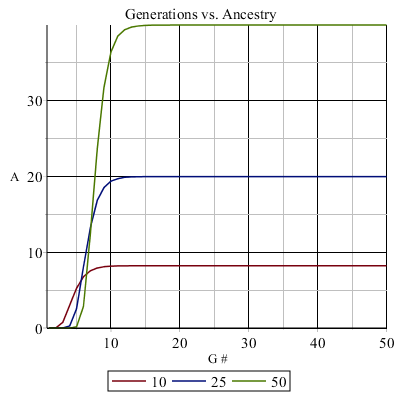
\includegraphics[scale=0.50]{Graph2.png}
		\caption{Cars=300}
		\label{fig:img2}
	\end{subfigure}
	\begin{subfigure}{0.50\textwidth}
		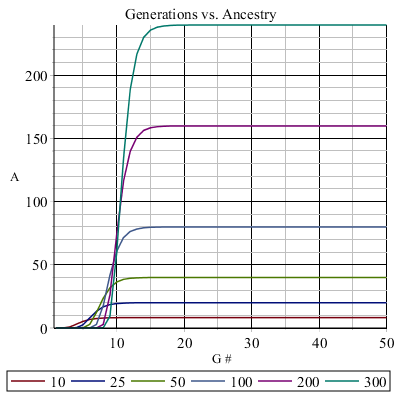
\includegraphics[scale=0.50]{Graph3.png}
		\caption{Cars = 400}
		\label{fig:img3}
	\end{subfigure}
\end{figure}

The next two figures show increasing car density over constant probability of deceleration. These tests were performed using 300 and 400 vehicles. In figure (\ref{fig:img2}) and (\ref{fig:img3}), red and black streaks are observed. These depict increased traffic at densities of 30\% and 40\%. Just as seen in the previous figure, streaks indicate consistent and inconsistent traffic. 

The differences across increasing densities show that traffic is generally consistent. Cases where multiple deadlocks merge into larger traffic jams can be observed. This can be explained by referring to the velocity rules. When a car decelerates, it will subsequently try to accelerate to the maximum velocity. 

\subsection{Probability Analysis}
\begin{figure}[h!]
	\centering
	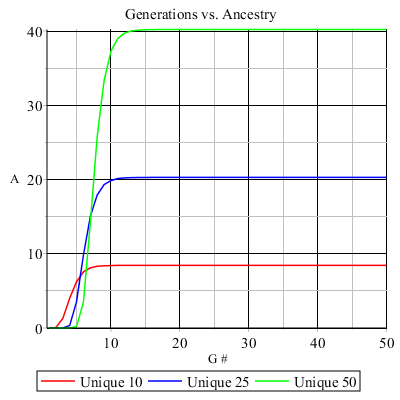
\includegraphics[scale=0.70]{Graph4.png}
	\caption{Cars = 100, Roads = 1000, Prob = 0.05}
	\label{fig:img4}
\end{figure}


In this section, the number of cars remains constant. The density is derived by equation (\ref{e3}). When the number of cars is constant and where the probability of deceleration changes, different results appear compared to a change in density .
\begin{figure}[h!]
	\caption{Roads = 1,000, Cars = 100}
	\begin{subfigure}{0.50\textwidth}
		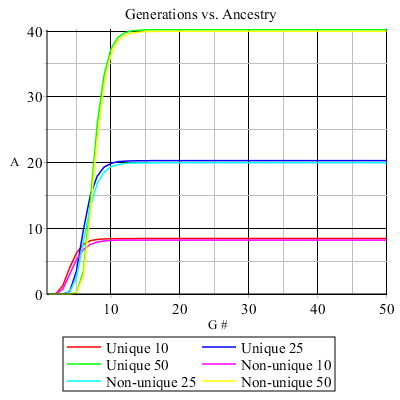
\includegraphics[scale=0.50]{Graph5.png}
		\caption{Probability = 0.25}
		\label{fig:img5}
	\end{subfigure}
	\begin{subfigure}{0.50\textwidth}
		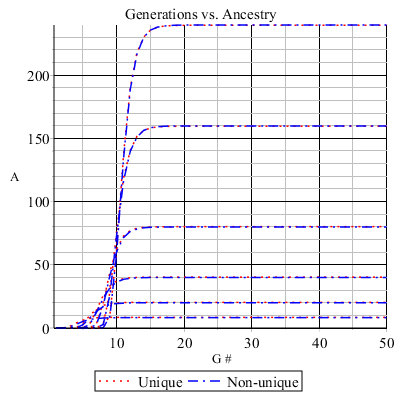
\includegraphics[scale=0.50]{Graph6.png}
		\caption{Probability = 0.40}
		\label{fig:img6}
	\end{subfigure}
\end{figure}
Comparing figure (\ref{fig:img1}) and (\ref{fig:img4}), the difference between the tests is 100 cars and a 10\% greater probability of deceleration. With fewer cars and an increased probability, the results show that road is traffic free. However, the characteristic observed in figure (\ref{fig:img4}) is not seen as frequently in the others is white streaking. These streaks represent space between cars. The figure also depicts a yellow noise. This results from random deceleration as seen in previous figures. It is important to note this difference as the decreased density creates better road conditions with a low deceleration probability. However, the yellow noise indicates road speeds are not always consistent.

Figures (\ref{fig:img5}) and (\ref{fig:img6}), depict the results of a simulation ran with 25\% and 50\% probabilities of deceleration. In the 25\% sample, more noise is observed and greater traffic consistency is seen as compared to figure (\ref{fig:img4}). The 50\% sample shows a different scenario. This simulation shows segments of road where deadlocks occurs. Fewer instances of traffic dissipation can be observed. Increased number of instances take more time to dissipate or persist outside these data. The two figures show that a 25\% probability reflect faster road velocities as compared to the 50\% figure. 

These results show that density affects road velocity more than random deceleration. With 100 cars and 50\% probability of deceleration, lower levels of traffic are observed compared to 200 cars with 5\% probability of deceleration. With these results it can be concluded that density has a greater affect on road conditions than deceleration probability. This is related to the length of road and number of cars present in the system. In a closed circuit, such as the one used in the simulation, it is evident that traffic can persist indefinitely. In the real world, it would be sufficient to state that traffic generally improves as the leading cars accelerate. 
\begin{wrapfigure}[15]{r}{0.475\textwidth}
	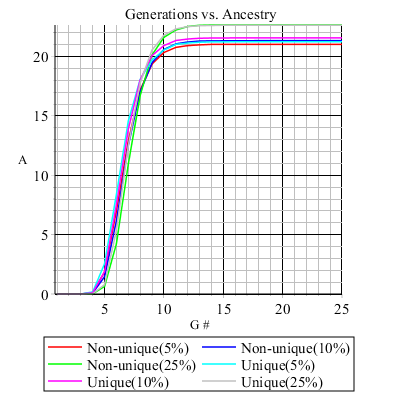
\includegraphics[scale=0.50]{Graph7.png}
	\caption{Cars = 200, Roads = 1,000, \newline Probability = $0.10 < P < 0.22$}
	\label{fig:img7}
\end{wrapfigure}
\subsection{Alternate Analysis}
\subsubsection{Normal Distribution Test}


In this section, an alternative test is performed. A normal curve equation is used to apply probability over a selected range of road. The peak of the curve is centered on road segment \#350. The minimum probability is 10\%, and the maximum is 22\%. 200 cars and 1,000 road segments are selected for this test.

Figure (\ref{fig:img7}), demonstrates the affect of the probability. Without the uniform distribution, used in previous tests, traffic patterns differ. The affect of applying the bell curve is similar to poor road conditions or an accident. Leading into the maximum, the traffic is most dense. 

Leading out of maximum value, conditions improve. The figure shows that the section of road from 400 to 800 is least dense. This can be seen in figure (\ref{fig:img7}) which shows that the majority of cars fall within segments 0 to 400 and 800 to 1,000. The cars between 400 and 800 have more room to accelerate and this results in better driving conditions within the range.

\subsubsection{Random Stop Test}

In this section, a car is selected and its maximum velocity is reduced to zero in the middle of the test. The parameters selected for the test were 200 cars, 1,000 road segments and a 10\% deceleration probability. The car selected halts for 20 steps in the test, beginning at $T=200$ and ending after $T=220$ at which point the car resumes a normal state.
\begin{wrapfigure}[15]{l}{0.475\textwidth}
	\includegraphics[scale=0.50]{Graph8.png}
	\caption{Cars = 200, Roads = 1,000, \newline Probability = $0.10$}
	\label{fig:img8}
\end{wrapfigure}
Figure (\ref{fig:img8}) depicts results of the test. It shows two reactions to the halt. Traffic conditions improve in front of the car, while the opposite is seen behind. This is an accurate representation of real world traffic caused by stopping cars.

This type of test shows best describes the real world equivalent of traffic lights. It shows the importance of timing stoplights appropriately. Several other tests were also performed that are not included in this report. These tests were run with increased duration. The results showed larger densities of traffic which persisted indefinitely.

\section{Technical Details}

This section describes details of how the tests described in this paper were performed and recorded. The tools used include maple and the programming language C$^\#$. Using these tools, the tests were carried out and performed multiple times. The best data were included to show the best results. 

Several programming techniques were used in the program to propagate results shown in figures throughout the paper. One technique used is known as a linked list\cite{linkedlist} which describes a sequence of objects that point to subsequent objects. However, the type of linked list technique used in this paper was circular. This describes a linked list that loops to the first value in the list from the last. 

A track describing cars and roads was programmed. When creating a test, the parameters of a track describe how the program should allocate the roads and cars. These parameters include the number of roads, cars and the probability of deceleration. Each road contains a link to the next road as well as a container for each car. Each car holds a constant for maximum and current velocity, and a link to the road in which it is associated.

The color used in the graphics was created using enumerated types\cite{Enumerated}. This is used to describe each of the colors by assigning it to an integer which is related to the velocity of a car. The integer can be converted to a word describing the color and the result is then used for the related figure. The color and data points are created in parallel.

When calculating the next position of a car, the linked list is used to determine the result. This interaction obeys rules described in the mechanics section of this paper. When the car is moved to the new location, the reference to the previous is removed.

When the probability is set at zero, the data changes considerably. The figures created from the data exhibited uniform color, occasionally with a large diagonal red stripe. This behavior is a product of the probability of deceleration. When randomized deceleration is removed, cars will space out and achieve a constant velocity that is uniform across all vehicles.


The function used for the normal distribution\cite{ND} test is described using equation:
\begin{align}
\notag
\frac{K}{\sigma\sqrt{2\pi}}e^{-\frac{(x-\mu)^2}{2\sigma^2}}
\end{align}
Within the programmed code, constants were supplied tuned for road lengths of 1000 and the peak at $x=350$. However, the equation was modified to contain a constant $K$. This is necessary in order to provide the appropriate range over the data.

\section{Conclusion}

This paper has described some of the mechanics of traffic and the interactions amongst vehicles. Using a simulation with a larger scope of data, the analysis could be improved. A major difference between this model and real world analysis is the roundabout property exhibited by the data. This model is sufficient for closed system testing however, large scale tests would be tailored to specific models.

Many of the mechanics observed in this paper accurately describe traffic in a real world scenario. When cars slow down, traffic density increases until an event occurs that changes the system. These conditions can be analyzed with mathematical models and predict outcomes based on real-time data. The model used for this paper lacks the detail used in real world models.

Drivers take for granted the research required to achieve understanding of road systems. Whether positioning traffic lights or preventing accidents, these models predict outcomes and help improve existing conditions. The affects of traffic can be seen further from origin either long-lasting or gradually dissipate. The study of these conditions are important in the real world since its implications can make or break road systems located near or far.








\newpage

\lstset{basicstyle=\footnotesize,breaklines=true}
\lstset{framextopmargin=50pt,frame=bottomline}

\section{C$^{\#}$ Code}
\lstinputlisting[caption=Tester.cs]{Tester.cs}
\lstinputlisting[caption=Car.cs]{Car.cs}
\lstinputlisting[caption=Road.cs]{Road.cs}
\lstinputlisting[caption=Track.cs]{Track.cs}
\newpage
\begin{thebibliography}{99}
\bibitem{linkedlist}"Linked List" Wikipedia: The Free Encyclopedia. Wikimedia Foundation, Inc. 9 Nov 2015. Web. 28 Nov 2015
\bibitem{Enumerated}"Enumerated Type" Wikipedia: The Free Encyclopedia. Wikimedia Foundation, Inc. 29 Nov 2015. Web. 28 Nov 2015
\bibitem{ND}"Normal Distribution" Wikipedia: The Free Encyclopedia. Wikimedia Foundation, Inc. 30 Nov 2015. Web. 1 Dec 2015

\end{thebibliography}

\end{document}
